\documentclass[a4paper]{article}

\usepackage[T1]{fontenc}
\usepackage[utf8]{inputenc}
\usepackage{polski}
\usepackage{graphicx}
\usepackage{hyperref}




\title{Programowanie Urządzeń Mobilnych \\ Laboratorium \\ \textbf{LISTA 2}}
\author{Rafał Lewandków}
\date{termin oddania: 27.11.2022}
\begin{document}
\maketitle
    

\section*{StudentCrime - 10 pkt}

Wykonaj prostą aplikację będącą zapisem wszystkich przewinień studentów. Aplikacja posiada jedną aktywność i dwa fragmenty. Pierwszy wyświetla \textbf{RecyclerView} wszystkich przewinień, drugi wyświetla widok szczegółowy przewinienia. Przechowujemy dane przewinienia - tytuł, treść, numer indeksu studenta, pole \textbf{Boolean} - \textbf{true} jeżeli przewinienie jest rozwiązane

\begin{itemize}
\item \textbf{3 pkt} -- Wykorzystując \textbf{Jetpack Navigation} przygotuj layout i nawigację aplikacji

\begin{figure}[h]
\centering
\caption{Layout pierwszego fragmentu}
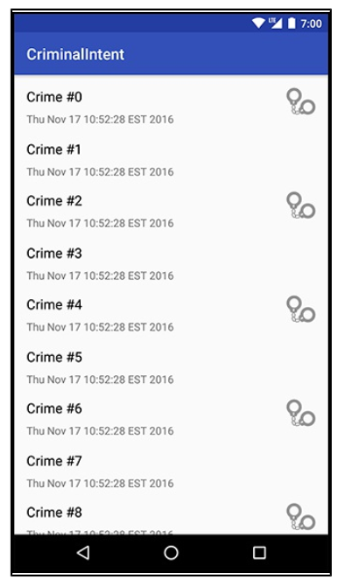
\includegraphics[scale=0.7]{l2.png}
\end{figure}

\begin{itemize}

\item \textbf{ListFragment} zawiera \textbf{RecyclerView}
\item layout elementu \textbf{RecyclerView} zawiera tytuł i \textbf{ImageView} z ikoną odpowiadającą polu \textit{isSolved}
\item \textbf{DetailFragment} zawiera wszystkie informacje o przewinieniu
\end{itemize}

\item \textbf{4 pkt} -- Dodaj \textbf{onClick} elementu  \textbf{RecyclerView} przez który przechodzimy do \textbf{DetailFragment} wyświetlającego informacje o wybranym przewinieniu

\item \textbf{3 pkt} -- Przygotuj model danych \verb+Crime+ i listę 20 przewinień - lista jest wyświetlana przy włączeniu aplikacji
\end{itemize}

\section*{OCENY}
Maxymalna liczba punktów: 10\\\
Oceny:\\
5.0 - 10 pkt\\
4.5 - 9 pkt\\
4,0 - 8 pkt\\
3,5 - 7 pkt\\
3,0 - 6 pkt
\end{document}

